% !TeX spellcheck = en_GB
% Template for ICASSP-2010 paper; to be used with:
%          mlspconf.sty  - ICASSP/ICIP LaTeX style file adapted for MLSP, and
%          IEEEbib.bst - IEEE bibliography style file.
% --------------------------------------------------------------------------
\documentclass{article}
\usepackage{amsmath,graphicx,02460}
\usepackage{amssymb}
\usepackage{bm}

\usepackage[dvipsnames]{xcolor}

\usepackage{pgf,tikz}
\usepackage{pgf-pie}
\usetikzlibrary{arrows}
\usetikzlibrary{decorations.markings}

\usepackage{url}
\allowdisplaybreaks
\PassOptionsToPackage{hyphens}{url}\usepackage{hyperref}
\def\UrlBreaks{\do\/\do-}

\toappear{02460 Advanced Machine Learning, DTU Compute, Spring 2022}


\newcommand{\code}[1]{{\texttt{\small#1}}}
\newcommand{\numberthis}{\addtocounter{equation}{1}\tag{\theequation}}
\newcommand{\acomm}[1]{\hspace{2.5cm}\text{#1}}
\newcommand{\low}[1]{\ensuremath{_\textup{#1}}}

\newcommand{\andim}{\textup{ and }}
\newcommand{\raq}{\Rightarrow\quad}
\newcommand{\lraq}{\Leftrightarrow\quad}
\newcommand{\qandq}{\quad\wedge\quad}
\newcommand{\qorq}{\quad\vee\quad}
\newcommand{\diff}[2]{\ensuremath{\frac{\md #1}{\md #2}}}
\newcommand{\md}{\ensuremath{\text{d}}}

\newcommand{\ctp}[1]{\ensuremath{\cdot10^{#1}}}
\newcommand{\reci}{\ensuremath{^{-1}}}
\newcommand{\twopow}{\ensuremath{^{2}}}
\newcommand{\re}[1]{\ensuremath{^{#1}}}

\newcommand{\me}{\ensuremath{\operatorname{e}}}
\newcommand{\eul}[1]{\ensuremath{\me^{#1}}}
\newcommand{\len}[1]{\ensuremath{\left\lvert#1\right\rvert}}
\newcommand{\half}{\ensuremath{\frac{1}{2}}}
\newcommand{\third}{\ensuremath{\frac{1}{3}}}
\newcommand{\fourth}{\ensuremath{\frac{1}{4}}}
\newcommand{\transpose}[1]{\ensuremath{#1^{\textup T}}}

\newcommand{\NN}{\ensuremath{\mathbb N}}
\newcommand{\ZZ}{\ensuremath{\mathbb Z}}
\newcommand{\QQ}{\ensuremath{\mathbb Q}}
\newcommand{\RR}{\ensuremath{\mathbb R}}
\newcommand{\CC}{\ensuremath{\mathbb C}}
\newcommand{\LL}{\ensuremath{\mathbb L}}
\newcommand{\PP}{\ensuremath{\mathbb P}}

\newcommand{\unit}[1]{\ensuremath{\:\text{#1}}}
\newcommand{\pro}{\ensuremath{\unit{\%{}}}}

%Kommandoer til ændring af ligestillingsmargner
\newcommand{\jl}[1]{\multicolumn{1}{l}{#1}}
\newcommand{\jc}[1]{\multicolumn{1}{c}{#1}}
\newcommand{\jr}[1]{\multicolumn{1}{r}{#1}}
\newcommand{\jls}[1]{\multicolumn{1}{l|}{#1}}
\newcommand{\jcs}[1]{\multicolumn{1}{c|}{#1}}
\newcommand{\jrs}[1]{\multicolumn{1}{r|}{#1}}

\title{20 Raspberry Pi's, One Model: Federated Learning On Real Hardware}
\name{Asger Laurits Schultz, Søren Winkel Holm, Gustav Lang Moesmand}
\address{Technical University of Denmark}
%
%
\begin{document}
%\ninept
%

\maketitle
%
\begin{abstract}
    Federated Learning (FL) is emerging as a essential mechanism for assuring user privacy in large-scale machine learning (ML) \cite{kai2021advances}.
    Important use-cases of this learning paradigm run on a federation of real-world user devices, but often in the literature, FL is simulated in an artificial computing cluster environment \cite{kai2021advances,mcmahan2017communication,lin2020ensemble}.
    Seeking to capture the unique FL problems and trade-offs when running on physical hardware, we install a network of 20 Raspberry Pi's acting as user devices.
    Using this experimental setup, we perform an empirical study of the influence of key hyperparameters of the FedAvg \cite{mcmahan2017communication} algorithm.
    For choosing the number of local epochs on clients, the physical timings allow us to identify a trade-off between spending time on communication and on local computation.
    Testing robustness both against imbalanced data across devices and the addition of rogue, noisy clients, we highlight the potential of using stronger aggregation schemes than averaging by implementing the FedDF \cite{lin2020ensemble} algorithm.
\end{abstract}
%
\begin{keywords}
    Federated Learning, Deep Learning, Privacy, Computer Vision
\end{keywords}


\section{INTRODUCTION}
\label{sec:intro}
Large-scale surveys have shown that the growing use of Artificial Intelligence (AI) has resulted in a widespread fear about loss of personal privacy \cite{beuc2020consumers, west2018survey}.
As a part of a general push towards safer AI, large tech companies such as Google and Apple have employed FL methods in cases such as Siri, Google Chrome and Gboard \cite{kai2021advances}.

The term FL covers the distributed ML setup where multiple clients collaborate in learning from local datasets which are not exchanged and where a central server aggregates updates \cite{kai2021advances, mcmahan2017communication}.
When the aggregation is performed by iteratively averaging weights from models each produced by training for a number local epochs on each client, the resulting FL algorithm is the formative \emph{FedAvg} \cite{mcmahan2017communication}.
To gain faster convergence and better data imbalance robustness, further aggregation methods have been developed, including the ensemble distillation algorithm \emph{FedDF} \cite{lin2020ensemble}, and we refer to Kairouz et al. for an overview of the field\cite{kai2021advances}.

Across this rich literature, many benchmarks of FL performance over algorithmic choices exist, but are often performed by simulating the federation on central compute clusters.
In this project, we seek to capture the unique hardware setup of FL use-cases such as smartphones where a number of computationally weak edge devices hold the data.
This is performed by performing local training of a convolutional neural network (CNN) on 20 Raspberry Pi devices over which CIFAR-10 \cite{alex2009learning} is divided, and aggregating these centrally using FedAvg.
The aim of the project is to investigate the impact of FedAvg hyperparameters including number of clients per communication round and local epochs on convergence time, analyze aggregation robustness against imbalanced and noisy data, and uncover performance bottlenecks and tradeoffs in the physical hardware setting.

\section{METHODS}%
\label{sec:methods}

\subsection{FL Methods}
We implemented FL by setting up $K$ clients each with a disjoint partition of the full training dataset.
A global model $\mathcal M_G$ was initialized and maintained on the central server, and for $L$ rounds, dubbed \emph{communication rounds}, $S \leq K$ clients were sampled, each receiving a copy of $\mathcal M_G$.
On each client, $E$ local epochs of gradient-based minibatch learning of the local dataset were performed before returning the updated model $\mathcal M_k$ to the server.

For FedAvg, the server aggregated the $S$ returned models by averaging over all model weights, yielding a new global model to be sent out for next communication round.

\begin{enumerate}
    \item TODO: Fed-DF. This is currently subject to change depending on the results
\end{enumerate}

\begin{figure}[ht!]
    \centering
    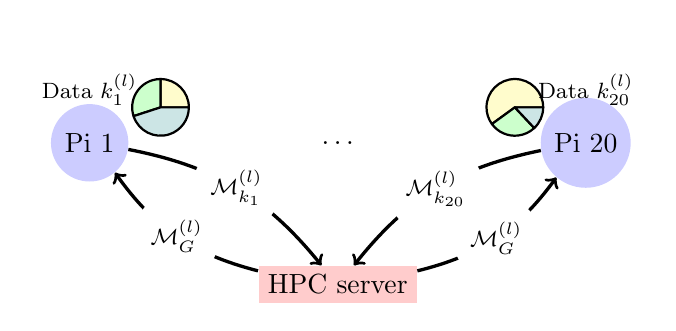
\begin{tikzpicture}[scale=.9,auto=center,every node/.style={circle}]

\tikzstyle{client}=[fill=blue!20];
\tikzstyle{server}=[fill=red!20,style=rectangle];
\tikzstyle{t}=[fill=red!0];

\node[server] (s) at (0,0) {HPC server};  
\node[client] (c1) at (-3.5,2)  {Pi $1$}; 
\node[t] (te) at (0, 2) {$\ldots$};
\node[client] (c2) at (3.5,2)  {Pi $20$};  



\path[->] (s) edge[very thick, bend left=20] node[midway, fill=white] {\footnotesize $\mathcal M_G^{(l)}$} (c1);
\path[->] (s) edge[very thick, bend right=20] node[midway, fill=white] {\footnotesize $\mathcal M_G^{(l)}$} (c2);

\path[->] (c1) edge[very thick, bend left=20] node[midway, fill=white] {\footnotesize $\mathcal M_{k_1}^{(l)}$} (s); 
\path[->] (c2) edge[very thick, bend right=20] node[midway, fill=white] {\footnotesize $\mathcal M_{k_{20}}^{(l)}$} (s); 

\pie[color={
    yellow!20,
    green!20,
    teal!20,
},
pos={-2.5,2.5},
radius=0.4,
hide number,
hide label]{25/L1, 30/L2, 45/L3};
\node (t1) at (-3.5, 2.75) {\footnotesize Data $k^{(l)}_1$};

\pie[color={
    yellow!20,
    green!20,
    teal!20,
},
pos={2.5,2.5},
radius=0.4,
hide number,
hide label]{60/L1, 27/L2, 13/L3};

\node (t2) at (3.5, 2.75) {\footnotesize Data $k^{(l)}_{20}$};



\end{tikzpicture}

    \caption{Our federated setup performing updates at communication round $l$ where Raspberry Pi 1 trains a local model on data partition $k_1$ (thus for round $l$, this device simulates client $k_1$) and Pi 20 trains as client $k_{20}$.}
    \label{fig:setup}
\end{figure}\noindent

\subsection{Physical Devices}
The project setup, shown on Figure \ref{fig:setup}, was divided into two pieces: A central high-performance cluster (HPC) and 20 Raspberry Pi 3B's, each with 1 GB memory and a quad-core 1.2 GHz CPU.
Crucially, the Pi's were located on a network separate from the HPC to simulate more realistic communication overhead.
The HPC server was responsible for aggregating the local models trained by the Pi's and evaluating the resulting global model.
The code was designed to not require physical devices, so experiments without physical timings interest could be run on an NVIDIA A100 for faster training time and a reduced power bill.

Every Pi ran a Flask server that received $\mathcal M_G^{(l)}$ every communication round $l$ and returned the trained local model along with telemetry data such as memory usage, which was an important consideration when running on such resource-limited devices.
The Flask server also had a route for sending commands to allow for primitive over-the-air-update functionality.
The Pi's were made accessible to the HPC using port-forwarding.

The Raspberry Pi setup able was designed to be able to run experiments where $K > 20$, that is maintaining more than 20 clients, each corresponding to a partition of the dataset, as long as no more than 20 clients were sampled each round ($S \leq 20$).
This was done by storing the entire dataset on each device and assigning each device to a client number, and thus a data partition, each communication round.

Each Pi was connected to a switch, which in turn was connected via cable to the router.
If the switches were turned off, the Pi's connected to the router via Wi-Fi, which allows for testing the impact of communication overhead in two cases: under relatively fast ethernet and relatively slow Wi-Fi.
For reference, the network used had a bandwidth of 100 Mbit/s both up and down, all of which would be utilized on ethernet, but only about 40\pro\ on Wi-Fi.

\subsection{Deep Learning Problem}
For an example learning problem, we chose the CIFAR-10 computer vision (CV) task of classifying $32\times 32$ images into object classes including bird, cat and airplane \cite{alex2009learning}.
Due to device memory limits, all images were greyscaled.

The training dataset contains 50K images of 10 equally common classes.
For the model $\mathcal M$, we chose a small network with two convolutional layers followed by two linear layers which is further detailed in Appendix \ref{app:model}.

Optimization for the $E$ local epochs on each device was performed by using the Adam optimizer \cite{kingma2015adam} with a learning rate $\eta$, which was decayed every local epoch: $\eta\leftarrow\gamma\eta, \gamma\le 1$.

\subsection{Data Imbalance and Noise}
\subsubsection{Dirichlet sampling}
The total training dataset was into $K$ evenly sized partitions among all the clients.

In practical, dataset class balance can rarely be assumed in FL setting \cite{kai2021advances}.
In order to simulate varying levels of imbalance, the Dirichlet distribution, $\operatorname{Dir}(\bm\alpha)$, was used.
The length of the parameter vector  $\bm\alpha$ corresponds to the number of labels, 10, and we let $\alpha_i=\alpha$.
Every sample $\bm\pi\sim\operatorname{Dir}(\bm\alpha)$ is a probability distribution over labels and $\alpha$ determines the uniformity of this distribution.
For $\alpha\to0$, one label dominates, where as for $\alpha\to\infty$, $\bm\pi$ will be increasingly uniform, as exemplified in Appendix \ref{app:dirplots}.
For $\alpha=1$, every possible $\bm\pi$ is equally likely.

$\bm\pi$ was sampled for every client, making the label distribution Dirichlet for every client.
To keep the client datasets disjoint while using a maximal part of the total dataset, we created and used a client-balancing Dirichlet sampling algorithm described in Appendix \ref{app:diralg}.

As a comparative baseline, we also simulate random partitions and denote this distribution scheme iid. following literature \cite{lin2020ensemble}.

\subsubsection{Noisy data}
To simulate the fact that some user devices can be unreliable, we tested the concept of noisy clients.
The training data on a noisy client had all labels replaced with randomly chosen classes, removing all signal.
We tested performance over the number of noisy clients $N_K\leq K$ to test for robustness against erroneous or even adversarial clients.

\subsection{Evaluation}
We perform experiments to test the effects of four variables: The number of clients sampled ($S$), the class balance (as controlled by $\alpha$ or iid.), the number of noisy clients ($N_K$), and the number of local epochs ($E$).

The experiments regarding clients sampled and local epochs are repeated on Raspberry Pi's both on ethernet and Wi-Fi.
Furthermore, the experiments regarding class balance and noisy clients are repeated using the FedDF algorithm.

All experiments used the baseline listed in Table \ref{tab:baseline} except for the parameter varied in each experiment.
These were chosen based on existing literature, in particular \cite{mcmahan2017communication,lin2020ensemble}, and on small pilot experiments.

\begin{table}[htb!]
    \centering
    \begin{tabular}{ccccccccc}
        $K$ & $S$ & $\alpha$ & $E$ & $L$ & $N_K$ & $B$ & $\eta$ & $\gamma$\\
        \hline
        40 & 20 & 1 & 20 & 20 & 0 & 16 & $5\ctp{-4}$ & $0.995$
    \end{tabular}
    \caption{Baseline parameters used for all experiments.
        Here, $B$ refers to the training batch size.}
    \label{tab:baseline}
\end{table}

\section{RESULTS}%
\label{sec:results}
Table \ref{tab:main} shows the results of different parameter choices using FedAvg after $L=20$ communication rounds.
% Redigér ikke tabel direkte, men redigér table_multirun.py
\begin{table}[htb!]
    \centering
    \begin{tabular}{llll}
       \hline
        \multicolumn{4}{c}{Local epochs ($E$)}\\
        1 & 10 & 20 & 40 \\
       \hline
        $48.0 \pm 0.9$ & $52.2 \pm 2.0$ & $37.6 \pm 2.4$ & $22.2 \pm 2.0$ \\
        \multicolumn{4}{c}{Clients sampled ($S$)}\\
        5 & 10 & 20 & 40 \\
       \hline
        $35.4 \pm 4.8$ & $37.4 \pm 2.6$ & $38.1 \pm 2.0$ & $38.1 \pm 2.5$ \\
        \multicolumn{4}{c}{Class balance ($\alpha$)}\\
        0.01 & 1.0 & 100.0 & iid \\
       \hline
        $10.3 \pm 0.6$ & $36.7 \pm 2.4$ & $42.6 \pm 3.4$ & $43.4 \pm 2.5$ \\
        \multicolumn{4}{c}{Noisy clients ($N_K$)}\\
        0 & 10 & 20 & 30 \\
       \hline
        $37.1 \pm 1.3$ & $14.0 \pm 2.1$ & $10.3 \pm 0.4$ & $10.6 \pm 0.8$ \\
\end{tabular}
    \caption{
    Final test accuracies [\%] of FedAvg models over $K=40$ clients after training for $L=20$ communication rounds.
    Each run is repeated five times to produce an approximate 95\%\ confidence interval.
    }
    \label{tab:main}
\end{table}

Figures \ref{fig:rpi-local-epochs} and \ref{fig:rpi-clients-per-round} show the four experiments run on the Raspberry Pi setup.
\begin{figure}[htb!]
    \centering
    \includegraphics[width=\linewidth]{imgs/time_avg_local_epochs_ethernet.pdf}
    \includegraphics[width=\linewidth]{imgs/time_avg_local_epochs_wifi.pdf}
    \caption{Effect of the number of local epochs using the Raspberry Pi setup on ethernet (top) and Wi-Fi (bottom).
    The lines show the mean accuracy of three repetitions, while the shaded areas outline the at any time best and worst of the repetitions.}
    \label{fig:rpi-local-epochs}
\end{figure}\noindent
    \begin{figure}[htb!]
    \centering
    \includegraphics[width=\linewidth]{imgs/time_avg_clients_per_round_ethernet.pdf}
    \includegraphics[width=\linewidth]{imgs/time_avg_clients_per_round_wifi.pdf}
    \caption{Effect of the number of clients per round using the Raspberry Pi setup on ethernet (top) and Wi-Fi (bottom).
    See Figure \ref{fig:rpi-local-epochs} for further description.}
    \label{fig:rpi-clients-per-round}
\end{figure}\noindent

\section{DISCUSSION}%
\label{sec:discussion}
\begin{enumerate}
    \item Add comments to Raspberry Pi Experiments: Use very short time on clients per round, but focus on local epochs.
        Comment on the fact that long-term behaviour is overfitting and more local epochs => more overfit.
        MAINLY: Focus the trade-off in number of local epochs in the first 20 minutes, where, especially on WiFi, 10 and 20 local epochs show their worth as there is more computation time.
    \item To talk about overfitting, use Figure \ref{fig:accuracy} or \ref{fig:accuracy2} and be amazed that FedAvg handles local overfitting so well.
    \item Comment on class balance and noisy clients using the repeated table numbers (wait for Fed-DF to finish before doing this).
    \item Discuss how realistic setup is.
\end{enumerate}
\begin{figure}[htb!]
    \centering
        \includegraphics[width=\linewidth]{imgs/accuracyE10.pdf}
    \caption{
        A training trajectory when recording running accuracies on each client in each communication round where each faint line correspond to $E=10$ local epochs performances of each of the $S=20$ sampled clients.
        For the baseline $E=20$ case, see Appendix Figure \ref{fig:accuracy2}.
    }
    \label{fig:accuracy}
\end{figure}\noindent


\vfill
\pagebreak

\bibliographystyle{IEEEbib}
\bibliography{references}

\appendix
\section{Model}
\label{app:model}
The model architecture is described below, listing the sequential operations in the foward pass.
\begin{table}[htb!]
    \centering
    \begin{tabular}{l|p{5cm}}
            Layer type & Hyperparameters\\
            \hline
            2D Convolution & 1 in-channel, 16 out-channels, $3\times 3$ kernel, stride of 1\\
            ReLU activation\\
            2D Convolution & 16 in-channels, 32 out-channels, $3\times 3$ kernel, stride of 1\\
            ReLU activation\\
            2D MaxPooling & $2\times 2$ kernel, stride of 2, no padding, dilation of 1\\
            Dropout & $p=25\%$\\
            Flattening\\
            Linear w. bias & $6,272$ features in, 64 features out\\
            ReLU \\
            Dropout & $p=50\%$\\
            Linear w. bias & 64 features in, 10 features out
        \end{tabular}
\end{table}\noindent
\section{The Dirichlet Distribution For Data Imbalance}
\subsection{Impact of Dirichlet $\alpha$}%
\label{app:dirplots}
\begin{figure}[htb!]
    \centering
        \includegraphics[width=0.49\linewidth]{imgs/splits(alpha=0.01)}
        \includegraphics[width=0.49\linewidth]{imgs/splits(alpha=1).pdf}
        \includegraphics[width=0.49\linewidth]{imgs/splits(alpha=100)}
        \includegraphics[width=0.49\linewidth]{imgs/splits(IID)}
    \caption{
        Example 10-class label distributions over 50 clients for each of the tested sampling paradigms, where each colour corresponds to a label and each row to a client.
    }
    \label{fig:splits}
\end{figure}\noindent


\subsection{Sampling Algorithm}%
\label{app:diralg}

\section{Further Result Plots}%

\begin{figure}[htb!]
    \centering
        \includegraphics[width=\linewidth]{imgs/accuracy.pdf}
    \caption{
        A version of \ref{fig:accuracy} with $E=20$.
        We note that the high value of local epochs results in a global model which is overfitting.
    }
    \label{fig:accuracy2}
\end{figure}\noindent




\end{document}
